\documentclass{beamer}

\usepackage{../macros}

\title{Array}

\begin{document}

\frame{
  \titlepage
}

\begin{frame}[fragile]{Array}
  
  \begin{block}{}
    \begin{itemize}
      \item A collection of items stored at contiguous memory locations
      \item Data structure to store multiple items of the same type
    \end{itemize}
  \end{block}
  
  \begin{block}{}
    \centering
    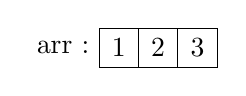
\begin{tikzpicture}[scale = 0.5]
      \draw (0, 0) rectangle (3, 1) 
        (1, 0) -- (1, 1)
        (2, 0) -- (2, 1);
      \draw (0.5, 0.5) node {1};
      \draw (1.5, 0.5) node {2};
      \draw (2.5, 0.5) node {3};
      \draw (0, 0.5) node[left] {arr :};
    \end{tikzpicture}
  \end{block}
  
  \begin{minipage}{0.48\textwidth}
    \begin{block}{In Python}
      \begin{lstlisting}[style=codePy]
arr = [1, 2, 3]
      \end{lstlisting}
    \end{block}
    
    \begin{block}{In R}
      \begin{lstlisting}[style=codeR]
arr <- c(1, 2, 3)
      \end{lstlisting}
    \end{block}
  
%    \begin{block}{In Shell}
%      \begin{lstlisting}[style=codeS]
%arr = (1 2 3)
%      \end{lstlisting}
%    \end{block}
  \end{minipage}\hfill
  \begin{minipage}{0.48\textwidth}
    \begin{block}{In C}
      \begin{lstlisting}[style=codeC]
int[] arr = {1, 2, 3};
      \end{lstlisting}
    \end{block}
  
    \begin{block}{In Java}
      \begin{lstlisting}[style=codeJ]
int[] arr = {1, 2, 3};
      \end{lstlisting}
    \end{block}
  \end{minipage}
\end{frame}

\begin{frame}{Exercise 1: Making Book}
  
\end{frame}

\begin{frame}{Exercise 2: It's a Murder}
  
\end{frame}

\end{document}
